% fig_ct_sweep.tex — CT saturation sweep (post-fix results)
% External FPR: Conv rises at eps=0.05; SAMBP=0.000 always
% Internal TPR: both Conv and SAMBP = 1.000 always (post-fix)
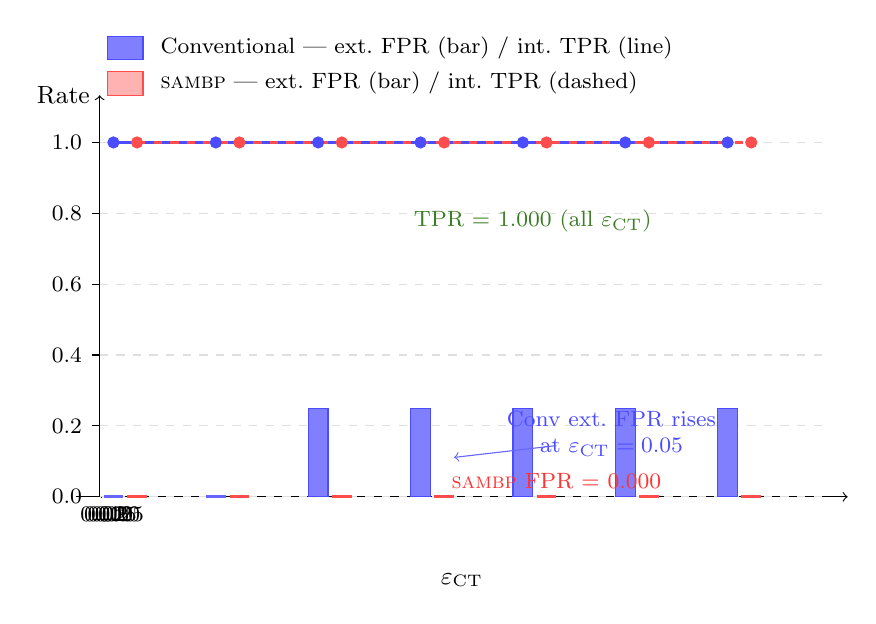
\begin{tikzpicture}

\def\H{4.5}
\def\DX{1.3}

% Axes
\draw[->] (0,0) -- (0,\H+0.6) node[left,font=\small]{Rate};
\draw[->] (-0.3,0) -- (9.5,0);

% Y ticks
\foreach \y/\val in {0/0.0, 0.9/0.2, 1.8/0.4, 2.7/0.6, 3.6/0.8, 4.5/1.0}{
    \draw (0,\y)--(-0.1,\y) node[left,font=\footnotesize]{\val};
    \draw[gray!25,dashed](0,\y)--(9.2,\y);
}

% X ticks
\foreach \i/\lbl in {0/0.00,1/0.02,2/0.05,3/0.10,4/0.15,5/0.20,6/0.25}{
    \pgfmathsetmacro\xp{\i*\DX + 0.6}
    \draw (\xp pt,0)--(\xp pt,-0.1pt)
          node[below,font=\footnotesize]{$\lbl$};
}
\node[font=\small,below=0.85cm] at (4.6,0) {$\varepsilon_{\rm CT}$};

%--------------------------------------------------------------------
% External FPR bars
% Conv heights (× 4.5 to map 0→0, 0.25→1.125)
%   eps:  0.00  0.02  0.05  0.10  0.15  0.20  0.25
%   conv: 0     0     1.125 1.125 1.125 1.125 1.125
%   sambp: 0 always

% i=0  eps=0.00  conv=0
\draw[blue!60,line width=1.2pt] (0.05,0)--(0.30,0);
\draw[red!70, line width=1.2pt] (0.35,0)--(0.60,0);

% i=1  eps=0.02  conv=0
\draw[blue!60,line width=1.2pt] (1.35,0)--(1.60,0);
\draw[red!70, line width=1.2pt] (1.65,0)--(1.90,0);

% i=2  eps=0.05  conv=1.125
\fill[blue!50] (2.65,0) rectangle (2.90,1.125);
\draw[blue!70] (2.65,0) rectangle (2.90,1.125);
\draw[red!70, line width=1.2pt] (2.95,0)--(3.20,0);

% i=3  eps=0.10  conv=1.125
\fill[blue!50] (3.95,0) rectangle (4.20,1.125);
\draw[blue!70] (3.95,0) rectangle (4.20,1.125);
\draw[red!70, line width=1.2pt] (4.25,0)--(4.50,0);

% i=4  eps=0.15  conv=1.125
\fill[blue!50] (5.25,0) rectangle (5.50,1.125);
\draw[blue!70] (5.25,0) rectangle (5.50,1.125);
\draw[red!70, line width=1.2pt] (5.55,0)--(5.80,0);

% i=5  eps=0.20  conv=1.125
\fill[blue!50] (6.55,0) rectangle (6.80,1.125);
\draw[blue!70] (6.55,0) rectangle (6.80,1.125);
\draw[red!70, line width=1.2pt] (6.85,0)--(7.10,0);

% i=6  eps=0.25  conv=1.125
\fill[blue!50] (7.85,0) rectangle (8.10,1.125);
\draw[blue!70] (7.85,0) rectangle (8.10,1.125);
\draw[red!70, line width=1.2pt] (8.15,0)--(8.40,0);

%--------------------------------------------------------------------
% Internal TPR lines (both at 1.000 = H=4.5)
\draw[blue!70,thick]
  (0.175,\H) -- (1.475,\H) -- (2.775,\H) -- (4.075,\H)
  -- (5.375,\H) -- (6.675,\H) -- (7.975,\H);
\draw[red!70,thick,dashed]
  (0.475,\H) -- (1.775,\H) -- (3.075,\H) -- (4.375,\H)
  -- (5.675,\H) -- (6.975,\H) -- (8.275,\H);

% Dots
\foreach \x in {0.175,1.475,2.775,4.075,5.375,6.675,7.975}{
    \filldraw[blue!70] (\x,\H) circle(2pt); }
\foreach \x in {0.475,1.775,3.075,4.375,5.675,6.975,8.275}{
    \filldraw[red!70] (\x,\H) circle(2pt); }

%--------------------------------------------------------------------
% Legend
\fill[blue!50](0.1,\H+1.05) rectangle (0.55,\H+1.35);
\draw[blue!70](0.1,\H+1.05) rectangle (0.55,\H+1.35);
\node[right,font=\footnotesize] at (0.65,\H+1.20) {Conventional — ext.\ FPR (bar) / int.\ TPR (line)};

\fill[red!30](0.1,\H+0.60) rectangle (0.55,\H+0.90);
\draw[red!70](0.1,\H+0.60) rectangle (0.55,\H+0.90);
\node[right,font=\footnotesize] at (0.65,\H+0.75) {\textsc{sambp} — ext.\ FPR (bar) / int.\ TPR (dashed)};

% Annotations
\node[font=\footnotesize,align=center,text=blue!70] at (6.5,0.80)
  {Conv ext.\ FPR rises\\at $\varepsilon_{\rm CT}=0.05$};
\draw[->,blue!60,thin] (5.8,0.65) -- (4.5,0.50);

\node[font=\footnotesize,text=OliveGreen] at (5.5,3.50) {TPR = 1.000 (all $\varepsilon_{\rm CT}$)};
\node[font=\footnotesize,text=red!80] at (5.8,0.20) {\textsc{sambp} FPR = 0.000};

\end{tikzpicture}
